% !TEX root = ../my-thesis.tex
%


\chapter{Attacking Fiat-Shamir with aborts over rings based signature schemes}
In this chapter we will describe our attack. First we introduce a previous attack from Espitau et al. \cite{espitau} in section \ref{sec:espitauattack}. %Then we will describe our attacker-model in detail in section \ref{sec:attackmodelgeneral}.
Then we will first describe the attack in general for lattice-based Fiat-Shamir with aborts over rings signature schemes in section \ref{sec:general}.
Finally we will describe the technical details to deploy the attack on Dilithium, qTESLA and BLISS in sections \ref{sec:attackdilithium}, \ref{sec:attackqtesla} and \ref{sec:attackbliss} respectively.
%In Section \ref{sec:general} we will describe our attack in general. Finally we will explain how this attack can be applied to Dilithium, qTesla and BLISS in section \ref{sec:attackdilithium}, \ref{sec:attackqtesla} and \ref{sec:attackbliss} respectively.

\section{Previous attack by Espitau et al.}
\label{sec:espitauattack}
Our attack is inspired by the fault attack and proposed countermeasures of Espitau et al. \cite{espitau}. They described their attack, among other schemes, against BLISS. They showed that a single fault during the signing process can reveal the secret key. In the following section we will describe their attack against BLISS.

\subsection{Attack idea}
\label{sec:espitau:idea}
The fault model the authors used was a loop-abort fault. % we described what this is in the backhround -> fault sectiom
A loop-abort fault is a fault intentionally induced by an attacker to prematurely end a loop, i.e. prevent a certain amount of iterations to be executed.  
The loop they targeted was the one sampling the coefficients of the masking polynomial $y_1$. Such a fault yields a masking polynomial with abnormal low degree. The degree is denoted by $m$. A BLISS signature is the triple $(c, z_1 = s_1 c + y_1, z_2^\dagger)$. A faulty signature with a faulty $y_1$ is all the information needed for performing this attack.

The important observation is that if we assume that $c$ is invertible, which is true with a high probability, then the vector $z_1 c^{-1}$ is close to a sublattice of $\mathds{Z}^n$. To be more precise we can see that
\[
z_1 c^{-1} - s_1 = c^{-1} y_1 = \sum_{i = 0}^{m-1}y_{1,i}c^{-1}x^i \mod{q}
\]
the sublattice $Λ$ is spanned by the vectors $w_i = y_{1,i}c^{-1}x^i$ for $i = 0, \ldots m - 1$ as well as the vectors $q\mathds{Z}^n$. The difference between $z_1 c^{-1}$ and that lattice is exactly $s_1$.

Because the dimension of that sublattice is still $n$, the secret cannot be recovered directly. But if we project the point $z_1 c^{-1}$ as well as the basis vectors of the sublattice $Λ$ to a subset of its rows, it still holds that the difference is the projected $s_1$. If the projection is chosen such that the degree is low enough, we can recover a part of $s_1$.  By choosing multiple such projections  we can eventually recover the entire secret polynomial and thus that the entire secret key.

Additionally the authors mention that the fault can also be of other nature. The attacker could for example target the memory where (part of) the masking vector is stored and fault it to zero  \cite[pp.~153--154]{espitau}.

%It is important to note here that it is crucial that we know which entries of the masking polynomial $y_1$ are faulty. So we need to know in which order the coefficients of $y_1$ are sampled as well as after what iteration the fault occurred. As pointed out in their countermeasures section this attack will not work if this information is not given because e.g. the coefficients are shuffled.
%In the next section we will describe attack that works efficiently even when this countermeasure is applied.

\subsection{Countermeasures}
\label{sec:countermeasure}
One of the proposed countermeasures by Espitau et al. is to generate the coefficients of $y_1$ in a random order \cite[p. 13]{espitau}. This prevents the attack as they do not know which of the $m < n$ vectors span the sublattice of interest, because they do not know which coefficients of $y_1$ are zero or not. This countermeasure can easily be added to an implementation because it is simple and fast. Using the  Fisher-Yates technique \cite{fisheryates} the shuffling can be done in $n$ iterations, i.e. linear complexity.

Furthermore they propose to add a check after sampling the coefficients of $y_1$. The idea is to check whether $y_1$ has too low degree. This would prevent their attack as they require $m$ to be at most around $100$ \cite[p.~151]{espitau}. The authors claim that if the signature process is aborted if more than $1/16$'th of the upper coefficients of $y_1$ are zero, the distribution of $y_1$ is skewed so little that it is statistically indistinguishable from the original one and thus the security proof of BLISS still holds \cite[p.~155]{espitau}. 




%Additionally we want to mention that the fault can also be of other nature. The attacker could for example target the memory where (part of) the masking vector is stored and fault it to zero  \cite{espitau}[pp.~153--154].
%While here we will always assume that faulted coefficients have the value $0$,as long as coefficients are faulted to a fixed known value, our attack also works, though some adjustments are needed. 


\section{General attack scheme}
\label{sec:general}
In this section we will describe our attack mostly signature scheme agnostic- First we will discuss our assumptions and important properties of the signatures in subsection \ref{sec:attack_prelim}, then we will describe our ILP in subsection \ref{sec:attackfinally} and finally we will describe an optimization in subsecton \ref{sec:prefilter}.


\subsection{Preliminaries}
This subsection will define our assumptions and notation and highlight two important properties of the signatures. These properties apply to all the three here discussed signatures.

\label{sec:attack_prelim}
\subsubsection{Assumptions and notation}
\label{sec:attackmodelgeneral}
The Fiat-Shamir with aborts signature schemes produce signatures in the form of $z = cs + y$ where $z$ is (part of) the signature (public), $s$ is (part of) the secret key (secret), $c$ is the commitment value (public) and $y$ is the masking vector (secret, (deterministically) random).

Here we will assume that the ring is $\mathcal{R}_q = \mathds{Z}_{q}[x] / (x^{n} + 1)$ with $n$ a power of two and $q$ an odd prime. Thus $z, s$ and $y$ are all elements in $\mathcal{R}_q$.

We assume an attacker who is able produce $σ$ signatures and in every signature he induces a loop-abort fault in the loop which samples the masking polynomial.  We assume that uninitialized $y$-coefficients are zero. Thus the faulted signature will have at least $1 \leq f \leq n$ zero coefficients in $y$ resulting in at most $m = n - f$ non-zero coefficients. As afterwards the coefficients are shuffled, he does not know where the zero coefficients are located.

While we here assume that a loop-abort fault will cause coefficients of $y$ to be zero, any kind of fault is theoretically possible, e.g. a fault in memory as already mentioned in section \ref{sec:espitau:idea}. Additionally, the faulted coefficients do not necessarily need to be zero, any other constant can works just as efficiently, though small modifications to the attack are needed.


\subsubsection{No modular reductions} \label{sec:nomod}
The commitment polynomials are sparse polynomials with coefficients which have small absolute values. While not sparse, the secret polynomials $s$ too have only coefficients with very small absolute value. Thus their product is below the modulus $q$ even when adding the masking polynomial $y$.  Thus during the computation of $z$ no modular reductions are performed or in other words, the operations can be seen as if they are performed in the ring $\mathcal{R} = \mathds{Z}[x] / (x^{n} + 1)$

\subsubsection{Linearity}
\label{sec:linearity}
To understand why the signature is linear we need to understand how we can describe the multiplication of the commitment polynomial $c$ and the secret polynomial $s$ in the Ring  $\mathcal{R} = \mathds{Z}[x]/(x^n+1)$  as a linear operation.
%We will assume that, this operation is performed in $\mathcal{R}$, as this is the case for all our signature schemes.

We can describe the multiplication as a matrix vector multiplication: The matrix is a quadratic $n \times n$ matrix $C$, which contains all $n$ negacyclic rotations (rotate, then negate) of the coefficient vector $c'$ of the commitment polynomial. The vector multiplied with $C$ is the coefficient vector $s'$ of the secret polynomial $s$ \cite[p.~1845]{negacyclic}.
Thus $Cs'$ is the coefficient vector of  $cs$ and together with the coefficient vector $y'$ of the masking polynomial $y$ we can write the entire signature as a linear equation system $z' = Cs' + y'$. 

%The  linear equation system has two classes of unknowns: The secret coefficients of the secret polynomial $s$, as well as the masking coefficients of the masking polynomial $y$.
%We know that a non-negligible amount of masking coefficients are zero. Our attack will thus not bother to recover the values of the masking coefficients, but instead only try to recover the information whether a masking coefficient is zero (most likely because of the fault) or not. Given that we have collected $\sigma$ signatures, we thus have to make $M = \sigma n$ boolean decisions whether a masking coefficient is zero or not. To summarize in our attack we will have to recover the a vector of size $n$ with entries in the range of the secret polynomial coefficients range as well as a boolean vector of size $M$.

\subsection{The attack}
\label{sec:attackfinally}
Let $M = σn$. Once we have gathered the faulted signatures we will use these signatures to construct $\dot{z} \in \mathds{Z}_q^{σ n}$ as the vector containing all $σ$ $z'$-vectors vertically stacked, $\dot{C} \in \mathds{Z}_q^{σ n \times n}$ as the matrix containing all  $σ$ $C$-matrices vertically stacked as well as $\dot{y} \in \mathds{Z}_q^{σ n}$ as the vector containing all $σ$ $y'$-vectors vertically stacked.

Now we can look at the bigger equation system $\dot{C}s' + \dot{y} = \dot{z}$.
We can not directly solve it because we do not know $\dot{y}$. Though we do know that $\dot{y}$ has a lot of zero entries, at least compared to a non-faulted version of this vector. The way we will look at this problem now is as follows: We will take the equation system  $\dot{C}s' = \dot{z}$ and say that it is \say{noisy}, i.e. that it has some rows $1 \leq i \leq M$ which are not \say{true} by which we mean that $\dot{y}_i \neq 0$.

In the following section we will refer to equations $\dot{C}_i s' = \dot{z}_i$ for which $\dot{y}_i = 0$ holds as \say{faulted equations} or \say{true equations} whereas for equations  $\dot{C}_i s' = \dot{z}_i$ for which $\dot{y}_i \neq 0$ holds we will refer to as \say{false equations} or \say{non-faulted equations}. 

To solve our the noisy linear equation system we will construct an instance of Marzougui's and Ulitzsch's \cite[pp.~46-47]{ulitzsch} ILP, which can classify true and false equations from one another, and solve the linear equation system for $s'$.


%The thinking now is not that if we knew which entries in $\dot{y}$ are zero, we could use the corresponding rows in $\dot{C}$ and entries in $\dot{z}$ to solve for $s'$ and recover the secret polynomial.
%To classify which entries in $\dot{y}$ are zero or not and recover the secret at the same time we will construct an instance of Marzougui's and Ulitzsch's \cite{ulitzsch}[pp.~46-47] ILP and try to solve it.
%Now we try to find a set $I \subseteq {1, \ldots, M}$ with $\lvert I \rvert \geq n$ which contains
%&Then our attack consists mainly of constructing an instance of Ulitzsch's \cite{ulitzsch}[pp.~46-47] ILP and solving it. 

\subsubsection{Variables}
\label{sec:ilpvars}
The ILP will use two classes of variables: $n$ variables in the same range as the coefficients of the secret polynomial $s$. We refer to them as the vector $\hat{s} \in \mathds{Z}_q^n$, Furthermore we will use $M$ boolean variables, We will refer to these variables as the vector $x \in \{0, 1\}^M$. 

%Ulitzsch's ILP is designed in a way that the objective will be maximized\footnote{with high probability (heuristically)} iff the $s$ vector is set to the secret polynomial coefficient vector and 
%for all $i \in {1, \ldots, M}$ $x_{i}$ will be $1$ iff the $(i \mod n)$'th $y$-coefficient of the $\lfloor i / n \rfloor$'th signature is zero. Or in other words: If $Y$ would be a vector containing all coefficients of the all $y$ polynomials obtained by the signatures, simply \say{stacked on one another}, $x_{i}$ will be $1$ iff the coefficient $Y_{i}$ is zero.

\subsubsection{Constraints and objectve}
Let  $K = \max_{z_{i}',C_{i}, s'}{\lvert z_{i}' - C_{i}s' \rvert}$. The ILP will aim to maximize $\sum_{i = 1}^M x_{i}$ while fulfillng the two constraints
%Besides the constraints for the domain of the vectors $\hat{s}$ and $x$ the ILP will have two important additional constraints. Here we choose $K$ to be $\max_{z_{i}',C_{i}, s'}{\lvert z_{i}' - C_{i}s' \rvert}$.
\begin{align}
	\label{constraint_leq}
	\dot{z} - \dot{C}\hat{s} & \leq K (1 - x) \\
	\label{constraint_geq}
	\dot{z} - \dot{C}\hat{s}  & \geq - K (1 - x)
\end{align}
in addition to  the constraints for the domain of the vectors $\hat{s}$ and $x$.

The two constraints can also be written in a more compact way:
\begin{align}
	\label{constraint_compact}
	 - K (1 - x) \leq \dot{z}- \dot{C}\hat{s}  \leq K (1 - x)
\end{align}

Let $s_{\text{min}}$ and $s_{\text{max}}$ be the lower and upper bound for the secret polynomial coefficients respecivley. Then the ILP with all its constraints can be formally defined as follows:

 % \[\text{maximize}\]
\begin{alignat}{3}
	&\text{maximize} &\text{\phantom{ii}}& \sum_{l = 1}^M x_{l} \\
	&\text{subject to} && \\
	%\label{constraint_leq}
	&&&\dot{z}_l - \dot{C}_l\hat{s}  \leq K (1 - x_l) &\text{\phantom{ii}}& \forall l \in \{1, \ldots, M \}\\
	%\label{constraint_geq}
	&&&\dot{z}_l - \dot{C}_l\hat{s}   \geq - K (1 - x_l) &&  \forall l \in \{1, \ldots, M \} \\
	&&&x_l \in \{0, 1\} && \forall l \in \{1, \ldots, M \}\\
	&&&\hat{s}_i \in  \mathds{Z} && \forall i \in \{1, \ldots, n \}\\
	&&&\hat{s}_i \leq  s_{\text{max}} && \forall i \in \{1, \ldots, n \}\\
	&&&\hat{s}_i \geq  s_{\text{min}} && \forall i \in \{1, \ldots, n \} 
\end{alignat}

\todo{A.: all in one formally ILP def}
\subsubsection{Reasoning}
The idea behind this ILP is that the objective will be maximized iff $\hat{s} = s'$ and the $x$-vector classifies the $\hat{y}$ coefficients correctly, i.e.
for all $i \in \{1, \ldots, M\}$ $x_{i}$ will be $1$ iff $\dot{y}_i = 0$ or in other words iff the $(i \bmod n)$'th $y$-coefficient of the $\lfloor i / n \rfloor$'th signature is zero.

To see why these two constraints do indeed help us to solve our problem we will look at what happens if the ILP-solver sets $x_{i} = 0$ or $x_{i} = 1$ for some $i \in \{1, \ldots, M\}$.

If $x_{i}$ = 0, the compact constraint \eqref{constraint_compact} will simplify to following.
\begin{alignat}{3}
	 &-K(1 - x_{i}) &&\leq \dot{z}_{i} - \dot{C}_{i}\hat{s}  &&\leq K(1 - x_{i}) \\
	 \label{alwaystrue}
	 \Leftrightarrow&- K &&\leq \dot{z}_{i} - \dot{C}_{i}\hat{s}  &&\leq K
\end{alignat}

This constraint is always true per our definition of $K$. In our use-case this means that when the ILP-solver sets $x_{i} = 0$ it effectively removes equation $i$ from our set of linear equations.
Note that the ILP-solver can always find a solution that will fulfill all constraints by setting $x = 0$, but this solution will not optimize the objective.  

If $x_{i}$ = 1 and $\hat{s} = s'$, the compact constraint \eqref{constraint_compact} will simplify to following.
\begin{alignat}{3}
&-K(1 - x_{i}) &&\leq \dot{z}_{i} - \dot{C}_{i}\hat{s}  &&\leq K (1 - x_{i}) \\
&-K(1 - 1) &&\leq \dot{z}_{i} - \dot{C}_{i}\hat{s}  &&\leq K (1 - 1) \\
\Leftrightarrow&0&&\leq \dot{z}_{i} - \dot{C}_{i}\hat{s}  &&\leq 0 \\
\Leftrightarrow&0 &&\leq  (\dot{C}_{i}s' + y'_{i}) - \dot{C}_{i}\hat{s}  &&\leq 0 \\
\Leftrightarrow&0&&\leq  \dot{y}_{i}  &&\leq 0 \\
 \Leftrightarrow&0&&=  \dot{y}_{i}   &&= 0
\end{alignat}
Thus, if the $y'_{i}$ is zero, most likely due to a fault, this constraint will be fulfilled.

If $x_1 = 1$ but $\hat{s} \neq s'$ this constraint could also be fulfilled.
We heuristically assume, supported by our successful simulations, that such events are very unlikely to maximize the objective and will this not be chosen by the ILP-solver.


\subsection{Pre-filtering equations without faults}
\label{sec:prefilter}


\begin{figure}%
	\centering%
	\begin{subfigure}{.5\textwidth}%
		\centering%
		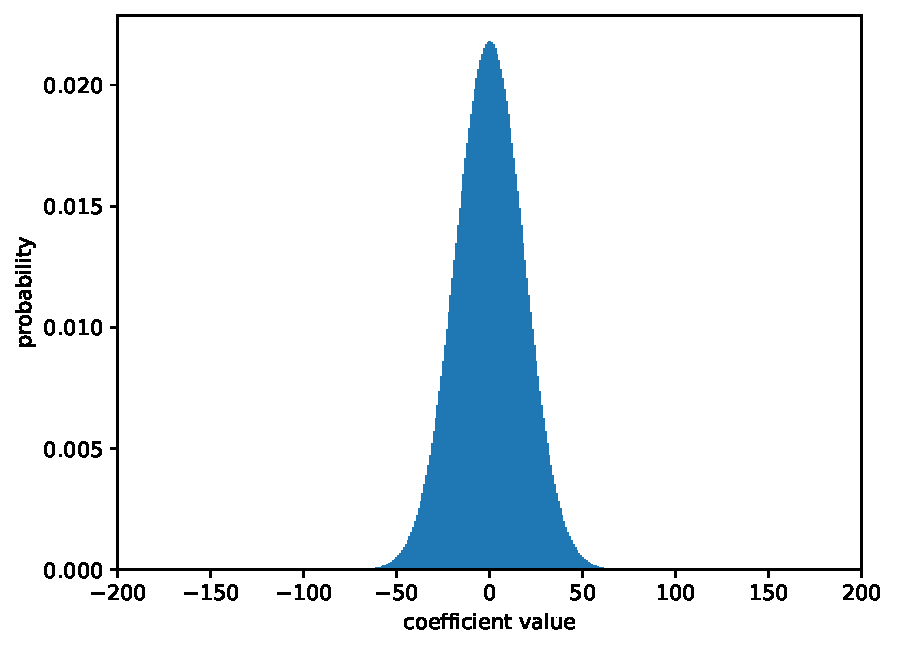
\includegraphics[width=.95\linewidth]{plots/dilithium_l3_cs_plot}%
		\caption{Dilithium (Security Level 3)}%
	\end{subfigure}%
	\begin{subfigure}{.5\textwidth}%
		\centering%
		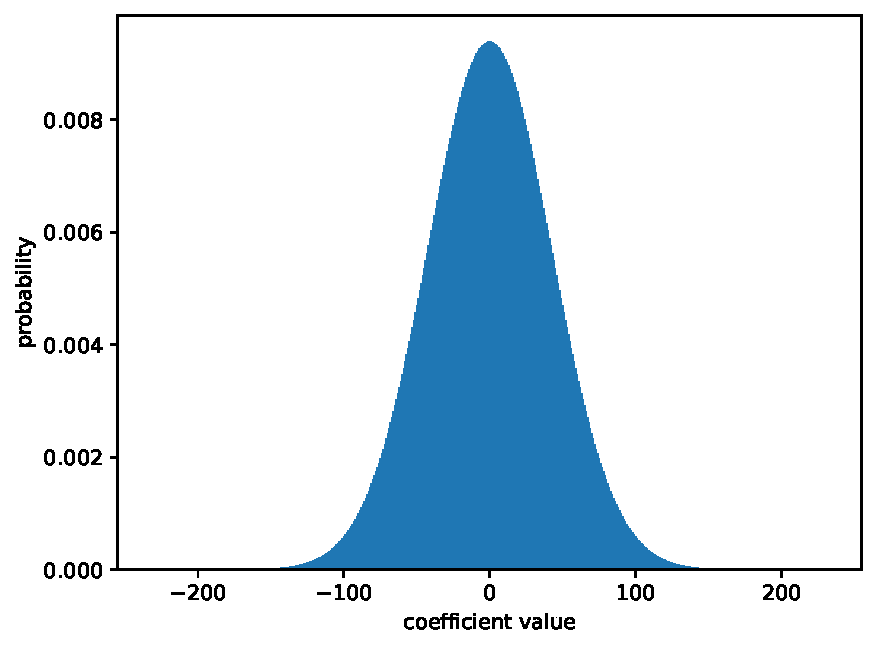
\includegraphics[width=.95\linewidth]{plots/qtesla_l3_cs_plot}%
		\caption{qTESLA (Security Level 1)}%
	\end{subfigure}\\\vspace{1em}%
	\begin{subfigure}{.5\textwidth}%
		\centering%
		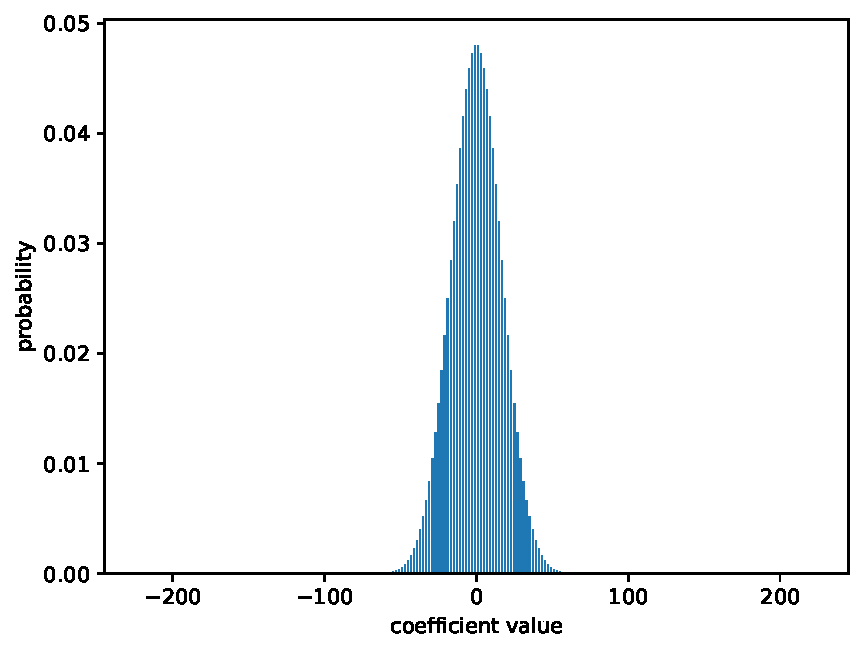
\includegraphics[width=.95\linewidth]{plots/bliss_l3_cs_plot}%
		\caption{BLISS (BLISS-III)}%
	\end{subfigure}%
%
	\caption{The distribution of a $cs$-coefficient (same as that of a faulted $z$-coefficient) for the different signature schemes. The plots for Dilithium and BLISS show the entire distributions. The plot for qTESLA shows the $6$-$σ$-interval of the $cs$ distribution.}
	\label{fig:csdist}
\end{figure}


The heavy lifting of classifying whether a coefficient of $y$ is zero or not is done by the ILP-solver.
Nevertheless for a certain set of equations we can say with ease that the corresponding $y$-coefficient can not be zero.
When a coefficient $y_{i}$ is zero we know that $z_{i} = (c s + 0)_{i}$. For all signature schemes we can give a bound $b$ to the maximum possible absolute value a coefficient of $cs$. Thus if $\lvert z_{i} \rvert>  b$, we know that $y_{i} \neq 0$ with a probability of $1$.

For improved performance we will thus remove any equations where we can tell, by using the aforementioned approach, that their corresponding $y$-coefficient is not zero. We do this before passing these equations to the ILP-solver. In practice this means removing the corresponding entry in the vector $z'$ and the corresponding row in the matrix $C$.

To go even further we can use a lower threshold $t < b$ to pre-filter our equations. Because for all three  signature schemes we know that the distribution of $cs$ has most of its probability mass close to zero, is symmetrical and thus has very little probability mass near the bounds $-b$ and $b$, this will filter out even more equations which are not affected by a fault. On the contrary we will also filter out some equations which were indeed affected by the fault increasing the amount of signatures we need. For a better visualization of the distributions see Figure \ref{fig:csdist}
\todo{maybe compare plots ot cs+y with y!=0}

%. Thus choosing a threshold $t < b$ we will thus need more signatures to perform our attack.
%This tradeoff between the amount of signatures required and the false-positive rate of the linear equation set we will be passing to the ILP-solver will be evaluated for Dilithium in section \ref{sec:evalthreshold}.


The metric we control by pre-filtering the equations is
%With pre-filtering we are able to control
the false-positive rate of our equation set. Here we classify an equation as being true, i.e. $y_{i} = 0$ or not. A true-positive classification would be if we classify an equation is faulted and it indeed is. A false-positive classification is when we classify an equation as faulted, although it actually is not. Thus the false-positive rate is ratio of the number false-positive classifications of our equations to the total number of equations. This number is an interesting metric for the efficiency of our attack as we will discuss later.
We are able to control this number by two parameters:
\begin{enumerate}
	\item the iteration number $m$, after which we induce a fault.
	\item the cutoff value $t$ we use for filtering
\end{enumerate}







\section{Attacking Dilithium}
\label{sec:attackdilithium}

In this section we will discuss the Dilithium signature scheme specific details for our attack.

\subsection{Implementation assumptions and attacker model}
First we assume that a big loop with $nl$ iterations will sample the coefficients for all $l$ polynomials with $n$ coefficients each in $\bm{y}$. Secondly we assume that the shuffling occurs throughout all the polynomials of the vector $\bm{y}$. This means that coefficients which where faulted to be zero located in the last polynomial may be shuffled to another polynomial, e.g. the first one.

We thus adjust our attacker model in the way that the attacker will induce a fault after the $1 \leq m \leq nl$ iteration in the loop which samples the coefficients of the masking polynomials.

\subsection{One ILP per polynomial}
The Dilithium signature scheme calculates the signature like follows:
\begin{align}
	\bm{z} = \bm{s}_{1} c + \bm{y}
\end{align}
Where $\bm{z}, \bm{s}_{1}, \bm{y} \in \mathcal{R}_q^{l}$ and $c \in \mathcal{R}_q$. We thus can not directly apply the attack mentioned before.
To still use our attack against Dilithium, let $\bm{z}_{i}, {\bm{s}_{1}}_{i}, \bm{y}_{i}$ be the $i$'th polynomial in the respective vectors for $1 \leq i \leq l$.
According to definition of $\bm{z}$ it holds for all $1 \leq i \leq l$ that $\bm{z}_{i} = c {\bm{s}_{1}}_{i} + \bm{y}_{i}$. Now, because $\bm{z}_{i}, c, {\bm{s}_{1}}_{i}, \bm{y}_{i} \in \mathcal{R}_q$ we can apply our attack for every $i$ to recover once secret polynomial of $\bm{s}_{1}$ at a time, eventually recovering the entire vector $\bm{s}_{1}$.

\subsection{Bound for the difference $z_{i}' - C_{i}s'$ and threshold $t$}
The coefficients of the commitment polynomial $c$ have at most an absolute value of $1$ which can occur at most $\tau$ times. The coefficients of the $\bm{s}_{1}$ polynomials have at most an absolute value of $\eta$. Thus we know that $\lvert  C_{i}s' \rvert \leq \tau \eta = \beta$. Finally the coefficients of the $\bm{y}$ masking polynomials have an absolute value of at most $\gamma_{1}$, thus $\lvert z'_{i} \rvert$ is at most $\tau \eta + \gamma_{1} = \beta + \gamma_{1}$. The absolute value of the difference is consequently $K = 2 \beta + \gamma_{1}$.

To filter equations we will use a threshold of $t = \beta$ as this is the upper bound for coefficients in $\bm{s}_{1}c$.% as we just discussed in the previous sections.

\subsection{Creating signatures using only \texorpdfstring{$\bm{s}_{1}$}{\textbf{s}1}}
In the Dilithium signature scheme $\bm{s}_{1}$ is only one part of the secret key. Our attack can not recover the second part of the secret key, $\bm{s}_2$, still $\bm{s}_{1}$ is enough information for an attacker to sign arbitrary messages. To sign arbitrary messages two different methods were previously presented. One by Bruinderink and Pessel \cite[pp.~33--34]{Groot_Bruinderink_Pessl_2018} and one by Ravi et al. \cite[pp.~12--13]{ravi_2018}. These signatures are indistinguishable from real ones when only given the public key. Only given the secret key we can distinguish the signatures created using only $\bm{s}_{1}$ from the ones created by someone with the entire secret key. 


\section{Attacking qTESLA}
\label{sec:attackqtesla}
Attacking qTESLA is straight forward because the qTESLA signature scheme strictly follows our general attack approach we presented in section \ref{sec:attackfinally}. Thus we only have to consider the maximum difference $z'_{i} - C_{i}s'$ and the appropriate threshold $t$.

\subsection{Bound for the difference $z_{i}' - C_{i}s'$ and threshold $t$}
\label{sec:qteslathreshold}
The polynomial $s$ has coefficients which follow the discrete gaussian distribution with standard deviation $\sigma$. This distribution is a long-tailed one and it can have theoretically infinitely large samples (coefficients). In practice discrete gaussian samplers have a parameter $\tau$ which defines a so called cutoff-value $\tau \sigma$, which limits the samples to be in the domain $[-\tau \sigma, \tau \sigma] \cap \mathds{Z}$. For our evaluation we choose $\tau = 6$ because this is the default one used in SageMath \cite{WEB:Sage}. Thus we can limit the domain of $s$ to be $[-\tau \sigma, \tau \sigma] \cap \mathds{Z}$.% This estimation is very conservative and better results may be possible by choosing a smaller $\tau$ when computing the threshold $t$.

The commitment value $c$ has exactly $h$ non-zero coefficients which are $-1$ or $1$ and the rest is zero. Thus we know that the polynomial $cs$ has coefficients in the range $[-h \tau \sigma, h \tau \sigma] \cap \mathds{Z}$.

The masking polynomial $y$ has per definition coefficients in the range $[-B, B] \cap \mathds{Z}$. Thus we can say that the coefficients of $z = y+cs$ are in the interval $[-B h \tau \sigma, B h \tau \sigma] \cap \mathds{Z}$.
Now looking at the difference $z'_{i} - C_{i}s'$ we know that that it's maximum absolute value is bounded by $2 h \tau \sigma + B$. Thus we choose $K = 2 h \tau \sigma + B$ and $t = h \tau \sigma$.


\section{Attacking BLISS}
\label{sec:attackbliss}
The BLISS \cite{bliss} signature scheme was first introduced by Léo Ducas et al. in 2013. With their novel rejection sampling algorithm and other modifications they were able to significantly reduce the standard deviation of their signatures and thus the signature size compared to other post-quantum secure schemes at that time. Their new rejection sampling algorithm is based on the bimodal gaussian distribution. This distribution is obtained in their scheme by choosing a random bit $b \in \{0, 1\}$ and computing a signature vector $z_{1} = y_{1} + (-1)^{b} s_{1}c$. The entire signature algorithm can be found in section \ref{sec:blissdesc}.


%\subsection{Special considerations}
Note that the previous two signature schemes do not use such a bit in their signature generation algorithms. To adapt our attack to BLISS we will have to include this bit of information in the ILP.
%For a single signature this is just a single bit of information, but as we require more signatures because we fault after more iterations the entropy will grow exponentially and the bits will be harder to recover.
%Despite this fact we were able to achieve good results for some of the proposed parameter sets of BLISS.
\todo{maybe add the out-commented paragraph to bliss results?}

\subsection{A modified ILP for BLISS}
Due to the random bit we now have three types of unknowns: The coefficients of the secret key polynomial $s_{1}$, the coefficients of the masking polynomial $y_{1}$ and the bit $b$.
Thus the ILP will use three classes of variables: In addition to $x$ and $\hat{s}$ we already described in the general ILP, we will have the binary variables $b_1, \ldots, b_σ \in \{0, 1\}$ to represent the random bit $b$.  

%Let $\hat{s} \in \{-2, -1, 0, 1, 2\}^{n}$ be the coefficient vector of $s_{1}$, let $x \in \{0, 1\}^{\sigma n}$ the binary / boolean vector which classifies whether a coefficient of one of the $y_{1}$'s is faulted or not just like we described in detail in section \ref{sec:ilpvars}. Finally let $b_{1},  b_{2}, \ldots, b_{\sigma} \in \{-1, 1\}^{\sigma}$ be the variables which describe the sign, which was induced by the bit $b$ ($(-1)^{b}$) for each signature .
%Here $\sigma$ denotes the amount of signatures we have acquired and $n=512$ for all BLISS parameter sets proposed by the authors.

Next will will define for all $1 \leq i \leq σ$ the vector $\vec{b}_i \in \{-1, 1\}^{n}$ as follows:%\footnote{Such a vector can not be straight forward be defined by a linear constraint, but with a small trick it is possible to construct something similar using a matrix vector product where the vector has $\sigma$ $\{0, 1\}$ entries which encode the signs.} \todo{probably explain the footnote in detail}
\begin{align}
	\vec{b}_i = (\overbrace{2(1-b_{i})-1, 2(1-b_{i})-1, \ldots, 2(1-b_{i})-1}^{n \text{ times}})^t\end{align}

This allows us to create the vector $\dot{b}$ which we define as all $\vec{b}_i$ vectors vertically stacked on one another, just like the definition of e.g.  $\dot{z}$.

Finally we can redefine the two constraints \eqref{constraint_leq} and \eqref{constraint_geq} of the ILP as follows,% Do note that additional constraints do define the domain of the different variables are required.
\begin{align}
	\label{constraint_leq_bliss}
	\dot{z} - \dot{b} \cdot C\hat{s} & \leq K (1 - x) \\
	\label{constraint_geq_bliss}
	\dot{z} - \dot{b} \cdot C\hat{s}  & \geq - K (1 - x)
\end{align}
where the $\cdot$ (dot) between $\dot{b}$ and $C\hat{s}$ denotes the entry-wise multiplication of the two vectors.


\subsection{Bound for the difference $z_{i}' - C_{i}s'$ and threshold $t$}
Let $d_{1} = \lfloor nδ_{1} \rfloor$ be the amount of $\pm1$ coefficients and $d_{2} =  \lfloor nδ_{2} \rfloor$ the amount of $\pm2$ coefficients in $s_1$.
Note that $c$ has exactly $κ$ coefficients with at most an absolute value of $1$ and the rest zero. Thus we maximize $C_i s'$ if all  $\pm2$-coefficient of $s_1$ match with non-zero coefficients of $C_i$ and the remaining $κ - d_2$ non-zero coefficients of $C_i$ match with the $\pm1$-coefficients in $s_1$. As for all parameter sets $κ > d_2$ holds, the bound for the absolute value of $C_i s'$ is  $2 d_{2} + κ - d_{2} = d_2 + k$,
%For all by the authors proposed parameter sets $C_{i}s'$ has at most an absolute value of $2 d_{2} + κ - d_{2} = d_2 + k$. \todo{why is that so, explain the calculation}
which we will use as the threshold.

The coefficients of $y_{1}$ follow the discrete gaussian distribution with a standard deviation $σ$. As already discussed in detail in section \ref{sec:qteslathreshold} we can limit the absolute values of the coefficients of $y_{1}$ to $τ σ$ with $τ = 6$. Thus we know that $\lvert z_{i}' \rvert \leq d_{2} + κ + τ σ$. Thus we choose $K = 2 (d_{2} + κ) + τ σ$.


\subsection{Recovering the entire secret key}
This attack will only recover the secret polynomial $s_{1}$ but not the second secret polynomial $s_{2}$. This is not a problem as $s_{1}$ is sufficient to recover the entire secret key: $s_2 = a_1 s_1 / 2 \bmod q$. This holds because:
\begin{align}
	a_{1}s_{1} / 2 = ((2g+1) / f)  s_{1} =  ((2g+1) / f)  f = (2g+1) f/f = 2g+1 = s_{2} \mod{q}
\end{align}






